% ============================================================
%  main.tex -- ADMS LLM Compression Slides
%  Metropolis Beamer Presentation
% ============================================================

\documentclass[aspectratio=169, 10pt]{beamer}

% ---------- Theme -------------------------------------------
\usetheme[progressbar=frametitle, block=fill, numbering=fraction]{metropolis}
\setbeamertemplate{section in toc}[sections numbered]
\setbeamertemplate{subsection in toc}[subsections numbered]

% ---------- Fonts -------------------------------------------
\usepackage[T1]{fontenc}
\usepackage[utf8]{inputenc}
\usepackage{FiraSans}
\usepackage{FiraMono}

% ---------- Math --------------------------------------------
\usepackage{amsmath, amssymb, mathtools}

% ---------- TikZ / pgfplots ---------------------------------
\usepackage{tikz}
\usetikzlibrary{arrows.meta, positioning, shapes.geometric, fit,
                backgrounds, calc, decorations.pathreplacing}
\usepackage{pgfplots}
\pgfplotsset{compat=1.18}

% ---------- Tables ------------------------------------------
\usepackage{booktabs, tabularx, multirow, colortbl}
\newcolumntype{Y}{>{\centering\arraybackslash}X}

% ---------- Graphics ----------------------------------------
\usepackage{graphicx}

% ---------- Bibliography ------------------------------------
\usepackage[backend=biber, style=authoryear-comp, maxcitenames=2,
            uniquelist=false, uniquename=false]{biblatex}
\addbibresource{refs.bib}
\setbeamertemplate{bibliography item}{}

% ---------- Utilities ---------------------------------------
\usepackage{appendixnumberbeamer}
\usepackage{qrcode}
\usepackage{hyperref}
\definecolor{mutedCite}{RGB}{120,88,55}
\hypersetup{
  colorlinks=true,
  linkcolor=.,
  citecolor=mutedCite,
  urlcolor=mLightBrown
}

% Keep in-slide citations visually secondary to slide content.
\AtEveryCite{\scriptsize}

% ---------- Custom commands ---------------------------------
\newcommand{\engine}[1]{\textbf{\textcolor{mLightBrown}{#1}}}
\newcommand{\codec}[1]{\texttt{#1}}
\newcommand{\metric}[1]{\textbf{\textcolor{mDarkTeal}{#1}}}
\newcommand{\plotsdir}{../adms_paper/plots}

% ---------- Metadata ----------------------------------------
\title{High-Throughput LLM-Based Compression}
\subtitle{Inference Engines and Entropy-Coding Optimizations}
\author[Adams et al.]{%
  \footnotesize
  David Adams\inst{1} \quad
  Luisa Neubauer\inst{2} \quad
  Ping-Lin Kuo\inst{2} \quad
  Mihail Stoian\inst{2}\\
  Thomas R\"uckstie\ss\inst{3} \quad
  Josif Grabocka\inst{2} \quad
  Renata Borovica-Gajic\inst{1} \quad
  Andreas Kipf\inst{2}
}
\institute[U Melbourne / UTN / Relaxed Constraints]{%
  \scriptsize
  \inst{1}The University of Melbourne
  \and \inst{2}University of Technology Nuremberg
  \and \inst{3}Relaxed Constraints
}
\date{ADMS 2026}

% ============================================================
\begin{document}
% ============================================================

\begin{frame}[plain]
  \titlepage
  \begin{tikzpicture}[remember picture,overlay]
    \node[anchor=south east, xshift=-0.6cm, yshift=0.45cm] at (current page.south east) {%
      \includegraphics[height=0.85cm]{260302_datasystems_logo_color.pdf}\hspace{0.8em}%
      \includegraphics[height=0.85cm]{danais-logo-light.pdf}%
    };
  \end{tikzpicture}
\end{frame}


\begin{frame}
  \frametitle{A summary of this Talk}
  \centering
  \definecolor{codecHuf}{HTML}{17BECF}
  \definecolor{codecLZ}{HTML}{D62728}
  \definecolor{codecSnappy}{HTML}{8C564B}
  \definecolor{codecOnPairSixteen}{HTML}{9467BD}
  \definecolor{codecFSST}{HTML}{7F7F7F}
  \definecolor{codecZstd}{HTML}{E377C2}
  \definecolor{codecToken}{HTML}{FF7F0E}
  \definecolor{codecOnPair}{HTML}{2CA02C}
  \definecolor{codecLLM}{RGB}{34,74,138}
  \begin{tikzpicture}[
    every node/.append style={text=black},
    codec label/.style={font=\scriptsize, fill=white, rounded corners=1.5pt,
      inner sep=1.5pt, line width=0.45pt},
  ]
    \begin{semilogyaxis}[
      width=0.96\textwidth,
      height=0.68\textheight,
      xmin=1.1, xmax=7.55,
      ymin=0.001, ymax=2000,
      xlabel={Compression ratio},
      ylabel={Compression throughput (MB/s)},
      xtick={1,2,3,4,5,6,7},
      ytick={0.001,0.01,0.1,1,10,100,1000},
      yticklabels={0.001,0.01,0.1,1,10,100,1000},
      grid=major,
      grid style={draw=black!15},
      axis line style={black!70},
      tick label style={font=\scriptsize},
      label style={font=\small},
      clip=false,
    ]
      % Encoding measurements reconstructed from Schmidt et al., Figure 13b.
      \addplot[only marks, mark=*, mark size=1.7pt, draw=codecHuf, fill=codecHuf]
        coordinates {(1.3898,1423.6)};
      \addplot[only marks, mark=*, mark size=1.7pt, draw=codecLZ, fill=codecLZ]
        coordinates {(1.8306,675.2)};
      \addplot[only marks, mark=*, mark size=1.7pt, draw=codecSnappy, fill=codecSnappy]
        coordinates {(1.8875,714.7)};
      \addplot[only marks, mark=*, mark size=1.7pt,
               draw=codecOnPairSixteen, fill=codecOnPairSixteen]
        coordinates {(2.2108,79.1)};
      \addplot[only marks, mark=*, mark size=1.7pt, draw=codecFSST, fill=codecFSST]
        coordinates {(2.0846,253.3)};
      % \addplot[only marks, mark=diamond*, mark size=2.1pt, draw=black!75, fill=black!75]
      %   coordinates {(2.72,104.93)};
      \addplot[only marks, mark=*, mark size=1.7pt, draw=codecZstd, fill=codecZstd]
        coordinates {(2.8594,546.7)};
      \addplot[only marks, mark=*, mark size=1.7pt, draw=codecToken, fill=codecToken]
        coordinates {(1.3804,323.9)};
      \addplot[only marks, mark=*, mark size=1.7pt, draw=codecOnPair, fill=codecOnPair]
        coordinates {(2.5945,94.2)};

      % Color-matched leaders reproduce the labeling style of the source figure.
      \draw[codecHuf] (axis cs:1.3898,1423.6) -- (axis cs:1.48,1650)
        node[codec label, draw=codecHuf, text=codecHuf, anchor=south west] {Huf};
      \draw[codecLZ] (axis cs:1.8306,675.2) -- (axis cs:1.58,480)
        node[codec label, draw=codecLZ, text=codecLZ, anchor=east] {LZ4};
      \draw[codecSnappy] (axis cs:1.8875,714.7) -- (axis cs:2.12,1150)
        node[codec label, draw=codecSnappy, text=codecSnappy, anchor=west] {Snappy};
      \draw[codecToken] (axis cs:1.5804,323.9) -- (axis cs:1.2,150)
        node[codec label, draw=codecToken, text=codecToken, anchor=west] {Token};
      \draw[codecFSST] (axis cs:2.0846,253.3) -- (axis cs:2.34,380)
        node[codec label, draw=codecFSST, text=codecFSST, anchor=west] {FSST};
      \draw[codecZstd] (axis cs:2.8594,546.7) -- (axis cs:3.12,1050)
        node[codec label, draw=codecZstd, text=codecZstd, anchor=west] {Zstd};
      \draw[codecOnPairSixteen] (axis cs:2.2108,79.1) -- (axis cs:1.48,47)
        node[codec label, draw=codecOnPairSixteen, text=codecOnPairSixteen,
             anchor=west] {OnPair16};
      \draw[codecOnPair] (axis cs:2.5945,94.2) -- (axis cs:2.25,25)
        node[codec label, draw=codecOnPair, text=codecOnPair, anchor=west] {OnPair+};
      % \draw[black!75] (axis cs:2.93,104.93) -- (axis cs:3.08,18)
      %   node[codec label, draw=black!75, text=black!75, anchor=west] {OptFSST};
      % \draw[codecHuf] (axis cs:2.0971,258.8) -- (axis cs:3.65,650)
      %   node[codec label, draw=codecHuf, text=codecHuf, anchor=west] {Token+Huf};
      % \draw[codecLZ] (axis cs:2.1816,247.3) -- (axis cs:3.65,250)
      %   node[codec label, draw=codecLZ, text=codecLZ, anchor=west] {Token+LZ4};
      % \draw[codecSnappy] (axis cs:2.1606,236.8) -- (axis cs:3.65,70)
      %   node[codec label, draw=codecSnappy, text=codecSnappy, anchor=west] {Token+Snappy};
      % \draw[codecZstd] (axis cs:2.4965,213.3) -- (axis cs:4.85,650)
      %   node[codec label, draw=codecZstd, text=codecZstd, anchor=west] {Token+Zstd};
      % \draw[codecOnPair] (axis cs:2.4950,85.5) -- (axis cs:4.85,180)
      %   node[codec label, draw=codecOnPair, text=codecOnPair, anchor=west] {Token+OnPair+};
      % Our end-to-end text8 measurements, Qwen2.5-0.5B on an A100.
      \draw[codecLLM, very thick, -{Latex[length=2mm]}]
        (axis cs:7.0482,0.0018) --
        node[pos=0.52, xshift=5mm, text=red!80!black, fill=white,
             inner sep=1.5pt, font=\small\bfseries] {$18.84\times$}
        (axis cs:7.0492,0.0345);
      \addplot[only marks, mark=*, mark size=1.7pt, draw=codecLLM, fill=codecLLM]
        coordinates {(7.0482,0.0018)};
      \addplot[only marks, mark=*, mark size=1.7pt, draw=codecLLM, fill=codecLLM]
        coordinates {(7.0492,0.0345)};
      \draw[codecLLM] (axis cs:7.0482,0.0018) -- (axis cs:6.72,0.0024)
        node[codec label, draw=codecLLM, text=codecLLM, anchor=east, align=right]
        {Unoptimized LLM\\0.0018 MB/s};
      \draw[codecLLM] (axis cs:7.0492,0.0345) -- (axis cs:6.92,0.055)
        node[codec label, draw=codecLLM, text=codecLLM, anchor=south east, align=right]
        {Optimized LLM \\0.0345 MB/s};
    \end{semilogyaxis}
  \end{tikzpicture}

  \vspace{-0.45em}
  \tiny\textcolor{codecOnPair}{\textbf{OnPair+ presentation:} Tue, Sep 1, 15:45--17:15, Grand Ballroom E -- Research 13: LLMs for Data Engineering}\par
  \tiny CPU: Schmidt et al.; OptFSST: mean over 92 columns; LLM: Qwen2.5-0.5B/A100/\texttt{text8}. Cross-system comparison. \parencite{schmidtAcceleratingStringHeavy2026,chehaidarOptFSST2026}
\end{frame}

\begin{frame}{Talk Roadmap}
  \tableofcontents
\end{frame}

% ============================================================
%  Section 1: Motivation
% ============================================================

\section{Motivation}

\begin{frame}{Text Is a First-Class Analytics Datatype}
  \begin{columns}[T, onlytextwidth]
    \begin{column}{0.48\textwidth}
      \begin{block}{Amazon Redshift fleet}
        \centering
        {\Huge 52.1\%}\\[0.4em]
        \small Stored columns observed as \texttt{varchar}\\[-0.1em]
        \scriptsize\parencite{vanrenenWhyTPCNot2024}
      \end{block}
    \end{column}
    \hfill
    \begin{column}{0.48\textwidth}
      \begin{block}{Snowflake workloads}
        \centering
        {\Huge 34\%}\\[0.4em]
        \small Aggregation inputs reported as text columns\\[-0.1em]
        \scriptsize\parencite{szlangWorkloadInsightsSnowflake2025}
      \end{block}
    \end{column}
  \end{columns}

  \vspace{1.0em}
  \begin{itemize}
    \item Analytical systems increasingly store and process large amounts of text.
    \item Compression already appears in production data pipelines, mostly through conventional codecs.
    \item Cold text is attractive: it is retained, moved, and scanned, but not constantly updated.
  \end{itemize}
\end{frame}

\begin{frame}{The Storage Codec Question}
  \begin{columns}[T, onlytextwidth]
    \begin{column}{0.44\textwidth}
      \textbf{Classical compressors}
      \begin{itemize}
        \item Extremely fast
        \item Cheap CPU deployment
        \item Moderate text compression ratios
        \item Mature in DBMS pipelines \parencite{zstd,fsst}
      \end{itemize}
    \end{column}
    \hfill
    \begin{column}{0.50\textwidth}
      \textbf{LLM-based compressors}
      \begin{itemize}
        \item Strong language priors
        \item High compression-ratio potential \parencite{llmzip,lossless_data_compression_llm}
        \item Require neural inference during encode and decode
        \item Need deterministic model and coder replay
      \end{itemize}
    \end{column}
  \end{columns}

  \vspace{0.9em}
  \begin{block}{Central systems question}
    Under which combinations of inference engine, hardware platform, and entropy-coding design can LLM compression become economically viable for analytical text storage?
  \end{block}
\end{frame}

\begin{frame}[standout]
  \Large Compression ratio is not enough.

  \vspace{1.0em}
  \normalsize
  A database codec has to balance storage footprint, ingestion throughput, and decode cost \parencite{Kipf2026WaitingTD}.
\end{frame}

% ============================================================
%  Section 2: Background
% ============================================================

\section{Background}

\newcommand{\codecell}[2]{%
  {\fontsize{17.5}{19}\selectfont\sffamily\bfseries\textcolor{mDarkTeal}{#1:}}%
  \hspace{0.08em}{\fontsize{7.8}{9.4}\selectfont\ttfamily\bfseries\textcolor{black!55}{#2}}%
}

\begin{frame}{Fixed-Length Codes: ASCII}
  \centering
  \resizebox{0.94\textwidth}{!}{%
  \begin{tikzpicture}
    \node[
      fill=mDarkTeal!3,
      draw=mDarkTeal!14,
      rounded corners=2pt,
      inner xsep=9pt,
      inner ysep=9pt
    ] {
      \begin{minipage}{0.98\textwidth}
        \centering
        {\fontsize{25}{27}\selectfont\sffamily\bfseries
          \textcolor{mDarkTeal}{ASCII $\longrightarrow$ }%
          \textcolor{mLightBrown}{8.0}%
          \hspace{0.18em}%
          \textcolor{mDarkTeal}{ bits/ch}}

        \vspace{0.75em}
        \setlength{\tabcolsep}{0pt}
        \renewcommand{\arraystretch}{1.95}
        \begin{tabular*}{\textwidth}{@{\extracolsep{\fill}}llllll}
          \codecell{a}{01100001} & \codecell{b}{01100010} & \codecell{c}{01100011} & \codecell{d}{01100100} & \codecell{e}{01100101} & \codecell{f}{01100110} \\
          \codecell{g}{01100111} & \codecell{h}{01101000} & \codecell{i}{01101001} & \codecell{j}{01101010} & \codecell{k}{01101011} & \codecell{l}{01101100} \\
          \codecell{m}{01101101} & \codecell{n}{01101110} & \codecell{o}{01101111} & \codecell{p}{01110000} & \codecell{q}{01110001} & \codecell{r}{01110010} \\
          \codecell{s}{01110011} & \codecell{t}{01110100} & \codecell{u}{01110101} & \codecell{v}{01110110} & \codecell{w}{01110111} & \codecell{x}{01111000} \\
          \codecell{y}{01111001} & \codecell{z}{01111010} & \codecell{0}{00110000} & \codecell{1}{00110001} & \codecell{2}{00110010} & \codecell{3}{00110011} \\
          \codecell{4}{00110100} & \codecell{5}{00110101} & \codecell{6}{00110110} & \codecell{7}{00110111} & \codecell{8}{00111000} & \codecell{9}{00111001}
        \end{tabular*}
      \end{minipage}
    };
  \end{tikzpicture}%
  }

  \vspace{0.2em}
  \small Every character gets the same 8-bit budget, regardless of how often it appears.
\end{frame}

\begin{frame}{Variable-Length Codes: Huffman}
  \centering
  \resizebox{0.94\textwidth}{!}{%
  \begin{tikzpicture}
    \node[
      fill=mDarkTeal!3,
      draw=mDarkTeal!14,
      rounded corners=2pt,
      inner xsep=9pt,
      inner ysep=9pt
    ] {
      \begin{minipage}{0.98\textwidth}
        \centering
        {\fontsize{25}{27}\selectfont\sffamily\bfseries
          \textcolor{mDarkTeal}{Huffman $\longrightarrow{\sim}$}%
          \textcolor{mLightBrown}{4.2}%
          \hspace{0.18em}%
          \textcolor{mDarkTeal}{ bits/ch}}

        \vspace{0.75em}
        \setlength{\tabcolsep}{0pt}
        \renewcommand{\arraystretch}{1.95}
        \begin{tabular*}{\textwidth}{@{\extracolsep{\fill}}llllll}
          \codecell{a}{1111} & \codecell{b}{010101} & \codecell{c}{01011} & \codecell{d}{11100} & \codecell{e}{011} & \codecell{f}{00100} \\
          \codecell{g}{110111} & \codecell{h}{0011} & \codecell{i}{1100} & \codecell{j}{110101010} & \codecell{k}{0010110} & \codecell{l}{11101} \\
          \codecell{m}{01000} & \codecell{n}{1011} & \codecell{o}{1010} & \codecell{p}{110110} & \codecell{q}{0010111010} & \codecell{r}{1001} \\
          \codecell{s}{1000} & \codecell{t}{000} & \codecell{u}{01001} & \codecell{v}{001010} & \codecell{w}{110100} & \codecell{x}{001011100} \\
          \codecell{y}{010100} & \codecell{z}{1101010111} & \codecell{0}{00101111} & \codecell{1}{11010100} & \codecell{2}{110101110} & \codecell{3}{110101111} \\
          \codecell{4}{1101011010} & \codecell{5}{1101011110} & \codecell{6}{1101010110} & \codecell{7}{0010111011} & \codecell{8}{1101011011} & \codecell{9}{110101100}
        \end{tabular*}
      \end{minipage}
    };
  \end{tikzpicture}%
  }

  \vspace{0.2em}
  \small Frequent symbols get shorter codewords; rare symbols pay more \parencite{Huffman1952AMF}.
\end{frame}

\begin{frame}{Arithmetic Coding: Compressing ``hello''}
  \centering
  \includegraphics[width=0.94\textwidth,height=0.76\textheight,keepaspectratio]{figures/tikz/ac_interval.pdf}

  \vspace{0.2em}
  \small The message is represented by a final interval; any binary fraction inside that interval decodes to the same text \parencite{rissanenArithmeticCoding1979}.
\end{frame}

\begin{frame}{Language Modeling Objective}
  \centering
  \Large
  \[
    P(x_{1:n}) = \prod_{t=1}^{n} P(x_t \mid x_{<t})
  \]

  \vspace{0.8em}
  \[
    \mathcal{L}_{\mathrm{NTP}}
      = - \sum_{t=1}^{n} \log P_\theta(x_t \mid x_{<t})
  \]

  \vspace{0.8em}
  \normalsize
  Next-token prediction trains the same conditional probabilities an entropy coder needs.
\end{frame}

\begin{frame}{LLM as Next-Token Prediction}
  \centering
  \resizebox{\textwidth}{!}{%
  \begin{tikzpicture}[
    node distance=0.9cm and 0.9cm,
    box/.style={draw, rounded corners=2pt, minimum width=2.15cm,
                minimum height=0.85cm, align=center, font=\small},
    arr/.style={-{Stealth[length=5pt]}, thick},
  ]
    \node[box, fill=blue!12, minimum width=2.55cm] (input) {Input tokens\\\texttt{the celtics are}};
    \node[box, fill=mLightBrown!20, minimum width=2.35cm, right=of input] (model) {Language model\\e.g., GPT};
    \node[box, fill=green!14, minimum width=3.0cm, right=of model] (dist) {Predicted distribution\\
      \texttt{playing}: 0.34\\
      \texttt{favored}: 0.18\\
      \texttt{in}: 0.08\\
      \ldots};
    \node[box, fill=orange!16, minimum width=2.7cm, right=of dist] (coder) {Arithmetic encoder\\actual token = \texttt{playing}};
    \node[box, fill=red!10, minimum width=2.45cm, right=of coder] (bits) {Compressed bitstream\\\texttt{101101...}};

    \draw[arr] (input) -- (model);
    \draw[arr] (model) -- (dist);
    \draw[arr] (dist) -- (coder);
    \draw[arr] (coder) -- (bits);

    \node[font=\scriptsize, align=center] at ($(model.south)+(0,-0.55)$)
      {predicts $P(\text{token}\mid\text{context})$};
    \node[font=\scriptsize, align=center] at ($(coder.south)+(0,-0.65)$)
      {encodes the observed next token\\using the predicted distribution};
  \end{tikzpicture}
  }

\vspace{0.6em}
\small Better predictions reduce bits; every token still requires deterministic model replay.
\end{frame}

\begin{frame}{Compression Is Not Ordinary Text Generation}
  \centering
  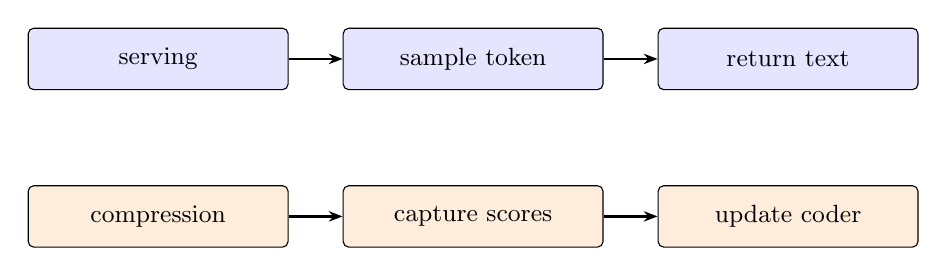
\begin{tikzpicture}[
    box/.style={draw, rounded corners=2pt, minimum width=3.3cm,
                minimum height=0.78cm, align=center, font=\small},
    arr/.style={-{Stealth[length=5pt]}, thick},
  ]
    \node[box, fill=blue!10] (serve) at (0,1.0) {serving};
    \node[box, fill=blue!10] (sample) at (4.0,1.0) {sample token};
    \node[box, fill=blue!10] (text) at (8.0,1.0) {return text};
    \draw[arr] (serve) -- (sample);
    \draw[arr] (sample) -- (text);

    \node[box, fill=orange!14] (comp) at (0,-1.0) {compression};
    \node[box, fill=orange!14] (scores) at (4.0,-1.0) {capture scores};
    \node[box, fill=orange!14] (ac) at (8.0,-1.0) {update coder};
    \draw[arr] (comp) -- (scores);
    \draw[arr] (scores) -- (ac);
  \end{tikzpicture}

  \vspace{0.8em}
  \small Generation engines optimize sampled-token serving; compression needs ordered scores or intervals for exact encode/decode replay \parencite{kwonEfficientMemoryManagement2023,zhengSGLangEfficientExecution2024}.
\end{frame}

% ============================================================
%  Section 2: Related Work
% ============================================================

\section{Related Work}

\begin{frame}{Related Work}
  \begin{columns}[T, onlytextwidth]
    \begin{column}{0.48\textwidth}
      \textbf{Neural compression}
      \begin{itemize}
        \item Neural predictors have long been combined with entropy coding \parencite{schmidhuberSequentialNeuralText1996}.
        \item DeepZip, DecMac, DZip, and TRACE improve modeling but keep inference cost central \parencite{goyalDeepZipLosslessData2019,liuDecMacDeepContext2019,goyalDZipImprovedGeneralpurpose2021,maoTRACEFastTransformerbased2022}.
      \end{itemize}
    \end{column}
    \hfill
    \begin{column}{0.48\textwidth}
      \textbf{LLM-based compression}
      \begin{itemize}
        \item LLMZip and later work show strong ratios from pretrained models \parencite{llmzip,lossless_data_compression_llm}.
        \item Recent systems work emphasizes practicality, latency, and coding precision \parencite{finezip,tacconelliNacrithNeuralLossless2026,Kipf2026WaitingTD}.
      \end{itemize}
    \end{column}
  \end{columns}
\end{frame}

\begin{frame}{The Systems Gap}
  \begin{columns}[T, onlytextwidth]
    \begin{column}{0.48\textwidth}
      \begin{block}{Compression literature}
        Usually asks: how good is the probability model, and how many bits does it save?
      \end{block}
      \small Classical references still define the codec baseline: Huffman coding, arithmetic coding, zstd, and FSST \parencite{Huffman1952AMF,rissanenArithmeticCoding1979,zstd,fsst}.
    \end{column}
    \hfill
    \begin{column}{0.48\textwidth}
      \begin{block}{LLM serving literature}
        Usually asks: how do we maximize generation throughput under serving workloads?
      \end{block}
      \small vLLM and SGLang optimize high-throughput LLM serving, but not the row-stable score-capture path required by entropy coding \parencite{kwonEfficientMemoryManagement2023,zhengSGLangEfficientExecution2024}.
    \end{column}
  \end{columns}

  \vspace{0.8em}
  \centering
  \small This work connects the two: model quality, engine behavior, and entropy-coder data movement.
\end{frame}

% ============================================================
%  Section 3: System and Optimizations
% ============================================================

\section{System}


\begin{frame}{Optimization Map}
  \centering
  \includegraphics[width=0.96\textwidth,height=0.78\textheight,keepaspectratio]{figures/tikz/optimization_legend.pdf}

  % \vspace{0.2em}
  % \small All three preserve the encoded probabilities. O1 and compressor-side O3 exploit that the input's next token is already known; O2 accelerates equivalent range-coder updates \parencite{Lam2015NumbaAL}.
\end{frame}

\begin{frame}{Experimental Setup}
  \small
  \begin{tabularx}{\textwidth}{lX}
    \toprule
    \textbf{Dimension} & \textbf{Configuration} \\
    \midrule
    Model & \texttt{Qwen/Qwen2.5-0.5B} \\
    Default hardware & Dual AMD EPYC Milan 7313, 512 GB DDR4, NVIDIA A100 40 GB SXM4 \\
    Datasets & \texttt{text8}, Python code from PyTorrent, Yelp Open Dataset records \\
    Default operating point & Batch size 256, context length 256, 100 retained tokens \\
    Metrics & Throughput in uncompressed MB/s; compression ratio as original/compressed size \\
    \bottomrule
  \end{tabularx}
\end{frame}

\begin{frame}{Three Datasets Cover Distinct Text Domains}
  \small
  \begin{tabularx}{\textwidth}{l>{\raggedright\arraybackslash}X>{\raggedright\arraybackslash}X}
    \toprule
    \textbf{Dataset} & \textbf{Content} & \textbf{Evaluation data} \\
    \midrule
    \texttt{text8} & English text extracted from Wikipedia & 100\,MiB \\
    PyTorrent & Python source code & First 100\,MiB \\
    Yelp Open Dataset & Structured business records & 150,346 records \\
    \bottomrule
  \end{tabularx}
  \vfill
  \tiny Datasets follow the evaluation corpus from prior work \parencite{Kipf2026WaitingTD}.
\end{frame}

\begin{frame}{Teacher-Forced Windows Amortize vLLM Scheduling}
  \centering
  \begin{tikzpicture}[scale=0.94,every node/.style={transform shape},
    req/.style={draw,rounded corners=2pt,minimum width=1.85cm,minimum height=0.7cm,align=center,font=\scriptsize},
    arr/.style={-{Stealth[length=5pt]},thick},
  ]
    \node[anchor=east,font=\small\bfseries] at (0.2,2.0) {one-token calls};
    \foreach \i/\x in {0/1.55,1/4.15,2/6.75,3/9.35} {
      \node[req,fill=red!9] (r\i) at (\x,2.0) {request + schedule\\score $t+\i$};
    }
    \draw[arr] (r0) -- (r1); \draw[arr] (r1) -- (r2); \draw[arr] (r2) -- (r3);

    \node[anchor=east,font=\small\bfseries] at (0.2,-0.25) {one window};
    \foreach \i/\x in {0/1.55,1/4.15,2/6.75,3/9.35} {
      \node[req,fill=blue!11] (s\i) at (\x,-0.25) {score $t+\i$\\force known token};
    }
    \draw[arr] (s0) -- node[above,font=\tiny] {KV state} (s1);
    \draw[arr] (s1) -- node[above,font=\tiny] {KV state} (s2);
    \draw[arr] (s2) -- node[above,font=\tiny] {KV state} (s3);
    \node[draw=mDarkTeal,very thick,rounded corners=2pt,fit=(s0)(s1)(s2)(s3),inner sep=6pt] {};
  \end{tikzpicture}

  % \vspace{0.7em}
  % \begin{block}{Why only vLLM?}
  %   vLLM's public path advances through a sampler and scheduler. Forcing lets one request traverse several known prefixes. Transformers already exposes a direct host-controlled token loop, so wrapping it in a generation request adds no benefit.
  % \end{block}
\end{frame}

\begin{frame}{Teacher-Forced Windows Amortize vLLM Scheduling}
  \centering
  \begin{tikzpicture}[
    box/.style={draw,rounded corners=2pt,minimum width=2.55cm,minimum height=0.9cm,align=center,font=\small},
    arr/.style={-{Stealth[length=5pt]},thick},
  ]
    \node[box,fill=blue!10] (score) at (0,1.3) {1. compute honest logits\\from current prefix};
    \node[box,fill=mLightBrown!15] (record) at (3.55,1.3) {2. record scores\\or target interval};
    \node[box,fill=green!12] (force) at (7.1,1.3) {3. force known $x_{t+1}$\\in the sampler};
    \node[box,fill=mDarkTeal!12] (advance) at (10.65,1.3) {4. append token\\advance KV cache};
    \draw[arr] (score) -- (record);
    \draw[arr] (record) -- (force);
    \draw[arr] (force) -- (advance);
    \draw[arr,rounded corners=5pt] (advance.south) -- ++(0,-0.75) -| node[below,pos=0.25,font=\scriptsize] {next internal decode step} (score.south);

    \node[draw,rounded corners=2pt,fill=black!4,align=center,font=\small,minimum width=5.35cm,minimum height=1.05cm] at (2.3,-1.15)
      {generation: sampled token\\chooses the next prefix};
    \node[draw,rounded corners=2pt,fill=mDarkTeal!8,align=center,font=\small,minimum width=5.35cm,minimum height=1.05cm] at (8.35,-1.15)
      {compression: observed file token\\chooses the next prefix};
  \end{tikzpicture}

  % \vspace{0.55em}
  % \small The score is captured \emph{before} forcing changes the sampler. KV caching avoids recomputing old keys and values, but each new position still runs the model.
\end{frame}

\begin{frame}{Windowing Raises vLLM Throughput $3.4\times$}
  \begin{columns}[T,onlytextwidth]
    \begin{column}{0.58\textwidth}
      \includegraphics[width=\textwidth]{\plotsdir/vllm_window_sweep_heatmap.pdf}
    \end{column}
    \hfill
    \begin{column}{0.37\textwidth}
      \vspace{0.55em}
      \begin{tikzpicture}
        \node[draw=mDarkTeal,very thick,rounded corners=3pt,fill=mDarkTeal!8,
          minimum width=4.2cm,minimum height=1.45cm,align=center]
          {\fontsize{28}{30}\selectfont\bfseries $3.43\times$\\[-0.05em]
           \small at the measured operating point};
      \end{tikzpicture}
      \vspace{0.7em}
      \small
      \begin{itemize}
        \item Gains concentrate at small and medium batches.
        \item Window 8 captures most of the benefit.
        \item Larger windows trade scheduling for memory.
      \end{itemize}
    \end{column}
  \end{columns}
  \vfill
  \tiny Qwen2.5-0.5B, vLLM, A100, \texttt{text8}; throughput in MB/s. Window 1 means one request per token.
\end{frame}

\begin{frame}[shrink=2]{Generation-Optimized Engines Expose the Wrong Interface}
  \centering
  \begin{tikzpicture}
    \begin{axis}[
      ybar,bar width=18pt,width=0.84\textwidth,height=0.45\textheight,
      ymin=0,ymax=0.038,ylabel={Compression throughput (MB/s)},
      symbolic x coords={Transformers,vLLM,TensorRT-LLM},xtick=data,
      tick label style={font=\small},label style={font=\small},
      grid=major,grid style={draw=black!13},scaled y ticks=false,
      yticklabel style={/pgf/number format/fixed,/pgf/number format/precision=3},
      nodes near coords,nodes near coords style={font=\scriptsize,/pgf/number format/fixed,/pgf/number format/precision=4},
    ]
      \addplot[fill=codecLLM!85,draw=codecLLM] coordinates {
        (Transformers,0.0344) (vLLM,0.0130) (TensorRT-LLM,0.0081)
      };
    \end{axis}
  \end{tikzpicture}

  \vspace{-0.2em}
  \small
  \begin{block}{High token serving throughput is not high compression throughput}
    Compression needs row-stable scores or intervals at every position. Scheduling, synchronization, and result reassembly become visible costs.
  \end{block}
  \vfill
  \tiny Qwen2.5-0.5B, batch 256, context 256, A100, \texttt{text8}; best comparable configuration per engine.
\end{frame}

% \begin{frame}{O1: Amortize the Request Boundary}
%   \centering
%   \begin{tikzpicture}[
%     reqbox/.style={draw,rounded corners=2pt,minimum width=1.8cm,minimum height=0.72cm,align=center,font=\scriptsize},
%     arr/.style={-{Stealth[length=5pt]},thick},
%   ]
%     \node[anchor=east,font=\small\bfseries] at (0.2,2.15) {baseline};
%     \foreach \i/\x in {0/1.5,1/4.2,2/6.9,3/9.6} {
%       \node[reqbox,fill=red!9] (r\i) at (\x,2.15) {request + schedule\\score $t+\i$};
%     }
%     \draw[arr] (r0) -- (r1);
%     \draw[arr] (r1) -- (r2);
%     \draw[arr] (r2) -- (r3);
%     \node[font=\scriptsize,text=red!70!black] at (5.55,1.38) {four request creations, schedules, and synchronizations};

%     \node[anchor=east,font=\small\bfseries] at (0.2,-0.35) {window $w=4$};
%     \node[reqbox,fill=blue!12] (s0) at (1.5,-0.35) {score $t$\\force $x_{t+1}$};
%     \node[reqbox,fill=blue!12] (s1) at (4.2,-0.35) {score $t+1$\\force $x_{t+2}$};
%     \node[reqbox,fill=blue!12] (s2) at (6.9,-0.35) {score $t+2$\\force $x_{t+3}$};
%     \node[reqbox,fill=blue!12] (s3) at (9.6,-0.35) {score $t+3$\\force $x_{t+4}$};
%     \draw[arr] (s0) -- node[above,font=\tiny] {KV state} (s1);
%     \draw[arr] (s1) -- node[above,font=\tiny] {KV state} (s2);
%     \draw[arr] (s2) -- node[above,font=\tiny] {KV state} (s3);
%     \node[draw=mDarkTeal,rounded corners=2pt,fit=(s0)(s1)(s2)(s3),inner sep=7pt,label={[font=\scriptsize,mDarkTeal]below:one vLLM request}] {};
%   \end{tikzpicture}

%   \vspace{0.8em}
%   \begin{block}{What O1 saves}
%     The same four model positions are evaluated. Windowing pays the fixed engine boundary once, rather than reducing the per-token transformer computation.
%   \end{block}
% \end{frame}


\begin{frame}{Multistreaming AC: Split the File into Row-Local Streams}
  \centering
  \begin{tikzpicture}[
    token/.style={draw,rounded corners=2pt,minimum width=0.75cm,minimum height=0.52cm,font=\scriptsize},
    box/.style={draw,rounded corners=2pt,minimum height=0.72cm,align=center,font=\small},
    arr/.style={-{Stealth[length=5pt]},thick},
  ]
    \node[font=\small\bfseries] at (1.45,3.2) {contiguous input rows};
    \node[font=\small\bfseries] at (6.0,3.2) {batched step $t$};
    \node[font=\small\bfseries] at (10.3,3.2) {independent coder states};

    \foreach \r/\y in {0/2.25,1/1.15,2/0.05} {
      \node[token,fill=mLightBrown!22] (seed\r) at (0,\y) {$x_{\r,1}$};
      \node[token,fill=blue!9] (a\r) at (0.95,\y) {$x_{\r,2}$};
      \node[token,fill=blue!9] (b\r) at (1.90,\y) {$\cdots$};
      \node[token,fill=blue!9] (c\r) at (2.85,\y) {$x_{\r,m_r}$};
      \node[box,fill=green!10,minimum width=2.15cm] (pred\r) at (6.0,\y) {$p_{\r,t}$ + true $x_{\r,t+1}$};
      \node[box,fill=mDarkTeal!12,minimum width=2.0cm] (coder\r) at (9.25,\y) {range coder $\r$};
      \node[box,fill=red!8,minimum width=1.6cm] (bits\r) at (11.85,\y) {bits $\r$};
      \draw[arr] (c\r) -- (pred\r);
      \draw[arr] (pred\r) -- node[above,font=\tiny] {$(\ell,h,T)$} (coder\r);
      \draw[arr] (coder\r) -- (bits\r);
    }

    \node[draw,rounded corners=2pt,fill=mLightBrown!10,align=center,font=\small,minimum width=4.1cm,minimum height=0.75cm] at (1.45,-1.25)
      {store the first token of each row\\to seed autoregressive decoding};
    \node[draw,rounded corners=2pt,fill=black!4,align=center,font=\small,minimum width=7.0cm,minimum height=0.75cm] at (9.1,-1.25)
      {parallel across rows; still sequential within each row};
  \end{tikzpicture}

  % \vspace{0.35em}
  % \small Row lengths and stream boundaries allow the independently encoded rows to be concatenated and reconstructed in original order.
\end{frame}

\begin{frame}{Multistream example: Two Rows, Two Bitstreams}
  \centering
  \begin{tikzpicture}[
    token/.style={draw,rounded corners=2pt,minimum width=0.62cm,minimum height=0.5cm,font=\small},
    box/.style={draw,rounded corners=2pt,minimum height=0.68cm,align=center,font=\small},
    arr/.style={-{Stealth[length=5pt]},thick},
  ]
    \node[anchor=east,font=\small\bfseries] at (-0.15,3.05) {input file};
    \foreach \x/\v in {0/A,0.72/B,1.44/A,2.16/C,2.88/A,3.60/B} {
      \node[token,fill=blue!9] at (\x,3.05) {\v};
    }
    \draw[very thick,mLightBrown] (1.80,2.65) -- (1.80,3.45);
    \node[font=\scriptsize,mLightBrown] at (1.80,2.43) {split into $B=2$ contiguous rows};

    \node[box,fill=mLightBrown!16,minimum width=1.65cm] (r0) at (0.45,1.25)
      {row 0\\\texttt{A B A}};
    \node[box,fill=mLightBrown!16,minimum width=1.65cm] (r1) at (0.45,-0.25)
      {row 1\\\texttt{C A B}};

    \node[box,fill=green!10,minimum width=3.55cm] (i0) at (4.1,1.25)
      {store seed \texttt{A}\\encode \texttt{B}: $[6,9)/10$\\encode \texttt{A}: $[0,7)/10$};
    \node[box,fill=green!10,minimum width=3.55cm] (i1) at (4.1,-0.25)
      {store seed \texttt{C}\\encode \texttt{A}: $[0,5)/10$\\encode \texttt{B}: $[2,9)/10$};

    \node[box,fill=mDarkTeal!13,minimum width=2.2cm] (c0) at (7.8,1.25)
      {coder state 0\\starts at $[0,255]$};
    \node[box,fill=mDarkTeal!13,minimum width=2.2cm] (c1) at (7.8,-0.25)
      {coder state 1\\starts at $[0,255]$};

    \node[box,fill=red!9,minimum width=1.65cm,font=\small\bfseries] (b0) at (10.75,1.25)
      {stream 0\\\texttt{11}};
    \node[box,fill=red!9,minimum width=1.65cm,font=\small\bfseries] (b1) at (10.75,-0.25)
      {stream 1\\\texttt{01}};

    \draw[arr] (r0) -- (i0);
    \draw[arr] (r1) -- (i1);
    \draw[arr] (i0) -- (c0);
    \draw[arr] (i1) -- (c1);
    \draw[arr] (c0) -- (b0);
    \draw[arr] (c1) -- (b1);

    \node[draw,rounded corners=2pt,fill=black!4,align=center,font=\scriptsize,
          text width=11.3cm,minimum height=0.82cm] at (5.45,-1.75)
      {payload = seeds \texttt{A,C} + stream lengths + stream 0 \texttt{11} + stream 1 \texttt{01}\\
       decode \texttt{A B A} and \texttt{C A B}, then join $\Longrightarrow$ \texttt{A B A C A B}};
  \end{tikzpicture}

  \vspace{0.15em}
  \scriptsize Toy alphabet $\{A,B,C\}$, frequency total $T=10$, and 8-bit coder state. Intervals come from each row's context-dependent model distribution; the displayed bits include the coder's terminating bit.
\end{frame}


\begin{frame}{Multistream makes the biggest difference}
  \centering
  \includegraphics[width=0.88\textwidth,height=0.66\textheight,keepaspectratio]{figures/tikz/bottleneck_shift.pdf}

  \vspace{0.15em}
  \begin{tikzpicture}
    \node[draw=codecBase,very thick,rounded corners=3pt,fill=red!6,
      minimum width=9.2cm,minimum height=0.8cm,align=center]
      {\textbf{97.1\%} of baseline wall time is arithmetic coding and score conversion};
  \end{tikzpicture}
  \vfill
  \tiny Qwen2.5-0.5B, Transformers, batch 256, A100, \texttt{text8}; end-to-end encode timing.
\end{frame}



\begin{frame}{Target-Interval Capture: Select Inside the Backend}
  \centering
  \begin{tikzpicture}[
    box/.style={draw,rounded corners=2pt,minimum height=0.78cm,align=center,font=\small},
    arr/.style={-{Stealth[length=5pt]},thick},
  ]
    \node[anchor=west,font=\small\bfseries] at (-1.6,2.75) {Baseline: dense scores cross the boundary};
    \node[box,fill=red!10,minimum width=3.2cm] (dense) at (0,1.75) {backend returns\\$B\times |V'|$ floats};
    \node[box,fill=red!10,minimum width=3.8cm] (host) at (4.4,1.75) {host softmax + integer counts\\prefix sum + target lookup};
    \node[box,fill=red!10,minimum width=2.6cm] (coder) at (8.8,1.75) {range-coder\\update};
    \draw[arr] (dense) -- (host);
    \draw[arr] (host) -- (coder);

    \node[anchor=west,font=\small\bfseries] at (-1.6,-0.1) {Target-Interval: select the known target before transfer};
    \node[box,fill=green!12,minimum width=3.2cm] (backend) at (0,-1.15) {backend softmax + counts\\prefix sum + target lookup};
    \node[box,fill=green!12,minimum width=3.8cm] (record) at (4.4,-1.15) {return $B$ records\\$(\ell,h,T,p_{target})$};
    \node[box,fill=mDarkTeal!12,minimum width=2.6cm] (coder2) at (8.8,-1.15) {range-coder\\update};
    \draw[arr] (backend) -- (record);
    \draw[arr] (record) -- (coder2);

    % \node[draw,rounded corners=2pt,fill=mLightBrown!12,align=left,font=\small,
    %       text width=10.9cm,inner sep=5pt] at (4.4,-2.75)
    %   {\textbf{Why integer counts?} Range coding updates an integer state, so encoder and
    %    decoder need the same cumulative bounds $(\ell,h,T)$. O3 moves this existing
    %    conversion; it does not add it.};
  \end{tikzpicture}
\end{frame}

\begin{frame}{Target-Interval Selection: One Row}
  \centering
  \begin{tikzpicture}[
    box/.style={draw,rounded corners=2pt,minimum height=0.72cm,align=center,font=\small},
    arr/.style={-{stealth[length=5pt]},thick},
  ]
    \node[font=\small\bfseries] at (1.75,3.0) {one model row};
    \node[box,fill=blue!10,minimum width=4.2cm] (probs) at (1.75,2.05)
      {alphabet $[a,b,c]$\\probabilities $[0.60,\,0.30,\,0.10]$\\known next file token: \texttt{b}};

    \node[font=\small\bfseries] at (7.25,3.0) {inside the inference backend};
    \node[box,fill=green!11,minimum width=3.75cm] (counts) at (6.2,2.05)
      {integer counts, $T=10$\\$[6,3,1]$\\CDF $[0,6,9,10]$};
    \node[box,fill=mLightBrown!16,minimum width=2.75cm] (select) at (10.25,2.05)
      {select \texttt{b}\\$[6,9)$};
    \draw[arr] (probs) -- (counts);
    \draw[arr] (counts) -- (select);

    \node[draw,rounded corners=2pt,fill=red!8,align=center,font=\small,
          minimum width=4.5cm,minimum height=1.05cm] (dense) at (2.25,-0.15)
      {\textbf{ordinary multistream handoff}\\transfer the dense row $[0.60,0.30,0.10]$\\host derives the target interval};
    \node[draw,rounded corners=2pt,fill=mDarkTeal!12,align=center,font=\small,
          minimum width=4.9cm,minimum height=1.05cm] (record) at (8.1,-0.15)
      {\textbf{target-interval handoff}\\transfer only $(\ell,h,T,p_{target})$\\$=(6,9,10,0.30)$};
    \draw[arr,red!65!black] (probs.south) -- (dense.north);
    \draw[arr,mDarkTeal] (select.south) -- (record.north);

    \node[box,fill=black!4,minimum width=6.6cm] (update) at (6.0,-1.75)
      {same row-local fastac coder: $[0,255]\rightarrow[153,229]$\\
       $low'=0+\lfloor 6\cdot256/10\rfloor$,\quad
       $high'=0+\lfloor 9\cdot256/10\rfloor-1$};
    \draw[arr] (dense.south) -- (update.north west);
    \draw[arr] (record.south) -- (update.north east);
  \end{tikzpicture}

  % \vspace{0.25em}
  % \small The integer range coder already needs $(\ell,h,T)$. O3 returns only that selected interval, removing the dense transfer and duplicate host work.
\end{frame}

\begin{frame}{Mutistream and Target Interval Raise Throughput $19\times$}
  \centering
  \begin{tikzpicture}
    \begin{axis}[
      xbar,bar width=11pt,width=0.83\textwidth,height=0.64\textheight,
      xmin=0,xmax=0.044,xlabel={Compression throughput (MB/s)},
      symbolic y coords={TensorRT target interval,TensorRT baseline,vLLM teacher-forced window,vLLM baseline,Transformers target interval,Transformers baseline},
      ytick=data,yticklabel style={font=\scriptsize},tick label style={font=\scriptsize},
      label style={font=\small},grid=major,grid style={draw=black!13},
      scaled x ticks=false,xticklabel style={/pgf/number format/fixed,/pgf/number format/precision=3},
      nodes near coords,nodes near coords style={font=\scriptsize,anchor=west,/pgf/number format/fixed,/pgf/number format/precision=4},
      enlarge y limits=0.10,
    ]
      \addplot[fill=codecLLM!85,draw=codecLLM] coordinates {
        (0.0018,Transformers baseline)
        (0.0347,Transformers target interval)
        (0.0031,vLLM baseline)
        (0.0116,vLLM teacher-forced window)
        (0.0020,TensorRT baseline)
        (0.0044,TensorRT target interval)
      };
    \end{axis}
  \end{tikzpicture}
  \vspace{-0.3em}

  \vfill
  \tiny Qwen2.5-0.5B, batch 256, context 128, A100, \texttt{text8}; relative gains use each engine's own baseline.
\end{frame}

% ============================================================
%  Section 4: Results
% ============================================================

\section{Results}

\begin{frame}{Result 1: Generation Engines Do Not Automatically Win}
  \small
  \begin{tabularx}{\textwidth}{llYYY}
    \toprule
    \textbf{Engine} & \textbf{Variant} & \textbf{MB/s} & \textbf{Ratio} & \textbf{Speedup} \\
    \midrule
    Transformers & + KV cache & \metric{0.0344} & 7.0492 & $1.00\times$ \\
    Transformers & No KV cache & 0.0030 & 7.0502 & $0.09\times$ \\
    vLLM & Default & 0.0130 & 7.0304 & $0.37\times$ \\
    TensorRT-LLM & Batch 256 & 0.0081 & 7.0499 & $0.023\times$ \\
    TensorRT-LLM & Batch 512 & 0.0065 & 7.9370 & $0.019\times$ \\
    \bottomrule
  \end{tabularx}

  \vspace{0.8em}
  \begin{block}{Interpretation}
    vLLM and TensorRT-LLM are excellent generation systems, but this workload exposes scheduling, synchronization, and score-capture costs that ordinary serving can hide \parencite{kwonEfficientMemoryManagement2023,Kipf2026WaitingTD}.
  \end{block}
\end{frame}

\begin{frame}{The Bottleneck Moves}
  \centering
  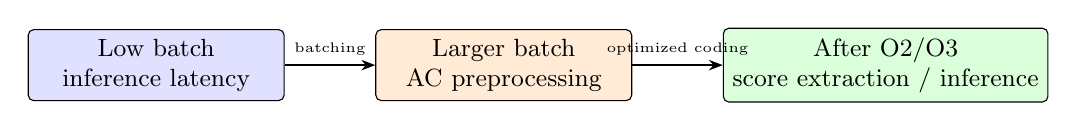
\begin{tikzpicture}[
    node distance=1.15cm,
    stage/.style={draw, rounded corners=2pt, minimum width=3.25cm,
                  minimum height=0.85cm, align=center, font=\small},
    arr/.style={-{Stealth[length=5pt]}, thick},
  ]
    \node[stage, fill=blue!12] (low) {Low batch\\inference latency};
    \node[stage, fill=orange!16, right=of low] (mid) {Larger batch\\AC preprocessing};
    \node[stage, fill=green!14, right=of mid] (high) {After O2/O3\\score extraction / inference};

    \draw[arr] (low) -- node[above, font=\tiny] {batching} (mid);
    \draw[arr] (mid) -- node[above, font=\tiny] {optimized coding} (high);
  \end{tikzpicture}

  \vspace{1.2em}
  \begin{itemize}
    \item Larger batches make GPU work more efficient, but expose arithmetic-coding cost.
    \item O2 reduces Python and range-coder overhead.
    \item O3 removes most probability-vector processing and transfer.
  \end{itemize}
\end{frame}

\begin{frame}{Result 2: Target-Interval Capture Dominates}
  \small
  \begin{tabularx}{\textwidth}{llYYY}
    \toprule
    \textbf{Engine} & \textbf{Configuration} & \textbf{MB/s} & \textbf{Rel. speedup} & \textbf{AC time} \\
    \midrule
    Transformers & Baseline AC & 0.0018 & $1.00\times$ & 97.1\% \\
    Transformers & + O3 & \metric{0.0347} & \metric{$18.96\times$} & \metric{1.0\%} \\
    Transformers & + O2 + O3 & 0.0345 & $18.84\times$ & 1.0\% \\
    \midrule
    vLLM & Baseline AC & 0.0031 & $1.00\times$ & 89.9\% \\
    vLLM & + O1 & \metric{0.0116} & \metric{$3.43\times$} & 9.2\% \\
    vLLM & + O3 & 0.0065 & $1.94\times$ & 3.0\% \\
    \midrule
    TensorRT-LLM & Baseline AC & 0.0020 & $1.00\times$ & 58.2\% \\
    TensorRT-LLM & + O3 & \metric{0.0044} & \metric{$2.18\times$} & 0.7\% \\
    \bottomrule
  \end{tabularx}
\end{frame}

\begin{frame}{Result 3: vLLM Needs Windowing}
  \begin{columns}[T, onlytextwidth]
    \begin{column}{0.56\textwidth}
      \includegraphics[width=\textwidth]{\plotsdir/vllm_window_sweep_heatmap.pdf}
    \end{column}
    \hfill
    \begin{column}{0.40\textwidth}
      \textbf{Takeaway}
      \begin{itemize}
        \item One next-token request per step pays too much fixed overhead.
        \item Teacher forcing collects several score vectors in one call.
        \item The benefit is largest at small-to-medium batch sizes.
        \item Window size $w=8$ is a practical operating point.
      \end{itemize}
    \end{column}
  \end{columns}
\end{frame}

\begin{frame}{Result 4: Context Length Mostly Buys Ratio}
  \small
  \begin{tabularx}{0.78\textwidth}{YYYY}
    \toprule
    \textbf{Context} & \textbf{Retain} & \textbf{MB/s} & \textbf{Ratio} \\
    \midrule
    32 & 16 & 0.0324 & 6.2288 \\
    64 & 32 & 0.0338 & 6.6592 \\
    128 & 64 & 0.0339 & 6.9239 \\
    \textbf{256} & \textbf{100} & \textbf{0.0337} & \textbf{7.0600} \\
    512 & 256 & 0.0349 & 7.1007 \\
    \bottomrule
  \end{tabularx}

  \vspace{0.8em}
  \begin{itemize}
    \item Throughput is nearly flat from context 64 to 512.
    \item Compression ratio improves, with diminishing returns after the first few hundred tokens.
    \item Context 256 is a memory-efficient default for this setup.
  \end{itemize}
\end{frame}

\begin{frame}{Result 5: LLM Ratios Are Strong, But Throughput Is Not}
  \small
  \begin{tabularx}{\textwidth}{lYYY}
    \toprule
    \textbf{Codec / encoding} & \textbf{MB/s} & \textbf{Ratio} & \textbf{Notes} \\
    \midrule
    Target interval AC & 0.0349 & \metric{7.1007} & LLM, optimized AC \\
    Bitpacked ranks & 0.0363 & 2.8735 & Simpler, much worse ratio \\
    Huffman ranks & 0.0359 & 6.1962 & No throughput advantage \\
    \midrule
    LZ4 & \metric{666.66} & 1.83 & CPU baseline \\
    zstd & \metric{586.70} & 3.06 & CPU baseline \\
    FSST & 294.11 & 2.08 & DB-centric baseline \\
    xz -9e & 1.34 & 4.30 & Stronger, slower baseline \\
    \bottomrule
  \end{tabularx}

  \vspace{0.5em}
  \small LLM compression currently trades orders of magnitude of throughput for substantially higher compression ratio. Classical baselines include zstd and FSST \parencite{zstd,fsst}.
\end{frame}

\begin{frame}{Dataset Sensitivity: Code Compresses Especially Well}
  \begin{columns}[T, onlytextwidth]
    \begin{column}{0.50\textwidth}
      \small
      \begin{tabularx}{\textwidth}{lYY}
        \toprule
        \textbf{Dataset} & \textbf{MB/s} & \textbf{Ratio} \\
        \midrule
        \texttt{text8} & 0.005436 & 7.739 \\
        \texttt{code} & 0.004132 & \metric{11.203} \\
        \texttt{Yelp} & 0.002490 & 7.028 \\
        \bottomrule
      \end{tabularx}
    \end{column}
    \hfill
    \begin{column}{0.44\textwidth}
      \begin{block}{Why this matters}
        Domain-structured text can be much more predictable than generic natural language.
      \end{block}
      \begin{itemize}
        \item Logs, code, schemas, and repeated business records are plausible targets.
        \item Fine-tuned or specialized models may shift the economics further \parencite{finezip}.
      \end{itemize}
    \end{column}
  \end{columns}
\end{frame}

% ============================================================
%  Section 5: Implications
% ============================================================

\section{Implications}

\begin{frame}{Where This Fits in a Database System}
  \begin{columns}[T, onlytextwidth]
    \begin{column}{0.48\textwidth}
      \begin{block}{Good fit}
        \begin{itemize}
          \item Cold or archival analytical text
          \item Write-once, read-rarely data
          \item Expensive storage or data movement
          \item Highly structured text or code corpora
        \end{itemize}
      \end{block}
    \end{column}
    \hfill
    \begin{column}{0.48\textwidth}
      \begin{block}{Poor fit today}
        \begin{itemize}
          \item Hot query paths
          \item High-throughput ingestion
          \item Frequent updates
          \item Latency-sensitive decompression
        \end{itemize}
      \end{block}
    \end{column}
  \end{columns}

  \vspace{0.8em}
  \centering
  \small The strongest current use case is not replacing zstd; it is compressing cold text when storage reduction dominates compute cost.
\end{frame}

\begin{frame}{Design Lessons for LLM Systems}
  \begin{enumerate}
    \item \textbf{Expose the right data.} Compression needs score or interval access, not sampled tokens.

    \vspace{0.4em}
    \item \textbf{Keep row order stable.} The entropy coder and decoder need deterministic, row-local replay.

    \vspace{0.4em}
    \item \textbf{Move work near inference.} Target-interval capture avoids exporting dense score tensors.

    \vspace{0.4em}
    \item \textbf{Batching changes the bottleneck.} Naive AC can dominate, but after O2/O3 the floor moves back to inference and score extraction.

    \vspace{0.4em}
    \item \textbf{Serving engines are not yet specialized for this.} High generation throughput does not imply high compression throughput.
  \end{enumerate}
\end{frame}

\begin{frame}{Future Work}
  \begin{columns}[T, onlytextwidth]
    \begin{column}{0.48\textwidth}
      \textbf{Model-side}
      \begin{itemize}
        \item Smaller or specialized compressors
        \item Domain fine-tuning for code, logs, and records
        \item Speculative or blockwise prediction
      \end{itemize}
    \end{column}
    \hfill
    \begin{column}{0.48\textwidth}
      \textbf{System-side}
      \begin{itemize}
        \item Native interval-capture APIs
        \item Lower-overhead stateful scheduling
        \item CPU-only paths with AVX-512 or other vector extensions
        \item Decode-aware cost models
        \item Integration with storage-tier policies
      \end{itemize}
    \end{column}
  \end{columns}
\end{frame}

% ============================================================
%  Section 6: Conclusion
% ============================================================

\section{Conclusion}

\begin{frame}{Future Work}
  \begin{columns}[T, onlytextwidth]
    \begin{column}{0.48\textwidth}
      \textbf{Model-side}
      \begin{itemize}
        \item Smaller or specialized compressors
        \item Domain fine-tuning for code, logs, and records
        \item Speculative or blockwise prediction
      \end{itemize}
    \end{column}
    \hfill
    \begin{column}{0.48\textwidth}
      \textbf{System-side}
      \begin{itemize}
        \item Native interval-capture APIs
        \item Lower-overhead stateful scheduling
        \item CPU-only paths with AVX-512 or other vector extensions
        \item Decode-aware cost models
        \item Integration with storage-tier policies
      \end{itemize}
    \end{column}
  \end{columns}
\end{frame}


\begin{frame}{Today the Fit Is Cold Database Text}
  \begin{columns}[T,onlytextwidth]
    \begin{column}{0.46\textwidth}
      \begin{block}{Plausible now}
        \begin{itemize}
          \item archival text and compliance logs
          \item write once, read rarely
          \item storage or transfer dominates
          \item structured domains such as code
        \end{itemize}
      \end{block}
    \end{column}
    \hfill
    \begin{column}{0.46\textwidth}
      \begin{block}{Not competitive now}
        \begin{itemize}
          \item hot scans and predicates
          \item high-throughput ingestion
          \item frequent updates
          \item latency-sensitive reads
        \end{itemize}
      \end{block}
    \end{column}
  \end{columns}

  \vspace{0.65em}
  \begin{tikzpicture}
    \node[draw=mDarkTeal,very thick,rounded corners=3pt,fill=mDarkTeal!7,
      minimum width=3.6cm,minimum height=1.15cm,align=center] at (2.0,0)
      {\Large\bfseries $7.7\times$ text\\[-0.1em]\scriptsize measured ratio};
    \node[draw=mDarkTeal,very thick,rounded corners=3pt,fill=mDarkTeal!7,
      minimum width=3.6cm,minimum height=1.15cm,align=center] at (6.0,0)
      {\Large\bfseries $11.2\times$ code\\[-0.1em]\scriptsize measured ratio};
    \node[draw=codecBase,very thick,rounded corners=3pt,fill=red!6,
      minimum width=3.6cm,minimum height=1.15cm,align=center] at (10.0,0)
      {\Large\bfseries $0.0345$ MB/s\\[-0.1em]\scriptsize optimized encode};
  \end{tikzpicture}
  \vfill
  \tiny Qwen2.5-0.5B, A100; ratios vary by dataset. Throughput value is \texttt{text8} encode only.
\end{frame}


\begin{frame}{Three Lessons for High-Performance LLM Compression}
  \begin{enumerate}
    \item \textbf{Measure the operator, not the model.} Generation throughput does not predict score-capture throughput.

    \vspace{0.35em}
    \item \textbf{Expose the value the consumer needs.} A target interval is cheaper to move than a vocabulary-wide score vector.

    \vspace{0.35em}
    \item \textbf{Evaluate both directions.} Encoder-only knowledge creates optimizations the decoder cannot share.
  \end{enumerate}

  \vspace{0.7em}
  \begin{columns}[c,onlytextwidth]
    \begin{column}{0.72\textwidth}
      \Large\textbf{Follow-up: Text Compression Through the Looking Glass}\\[0.35em]
      \normalsize\href{https://utndatasystems.github.io/blog/2026/text-compression/}{utndatasystems.github.io/blog/2026/text-compression/}\\[0.65em]
    \end{column}
    \begin{column}{0.24\textwidth}
      \centering
      \qrcode[height=2.2cm]{https://utndatasystems.github.io/blog/2026/text-compression/}
    \end{column}
  \end{columns}
\end{frame}


\appendix


\begin{frame}[allowframebreaks]{References}
  \scriptsize
  \printbibliography[heading=none]
\end{frame}

\begin{frame}[standout]
  \Large Questions

  \vspace{1.2em}
  \normalsize
  David Adams\\
  \href{mailto:david.adams1@student.unimelb.edu.au}{david.adams1@student.unimelb.edu.au}

  \vspace{1.1em}
  \begin{minipage}{0.52\textwidth}
    \centering
    \begin{minipage}[t]{0.48\textwidth}
      \centering
      \qrcode[height=1.45cm]{https://github.com/Dadams2/ADMS_2026_LLM_Compression}\\[0.35em]
      \small Slides and code
    \end{minipage}
    \hfill
    \begin{minipage}[t]{0.48\textwidth}
      \centering
      \qrcode[height=1.45cm]{https://wa.me/qr/RKT2JZPJOPGZH1}\\[0.35em]
      \small Talk to me!
    \end{minipage}
  \end{minipage}
\end{frame}

% ============================================================
\end{document}
